\section{Выпуклые и вогнутые функции. Переформулировки определения выпуклости \href{https://youtu.be/CAxh8kYEOlQ?t=2655}{\Walley}}
\begin{conj}
    $f: \langle a, b \rangle \longrightarrow \R \quad$ выпуклая, если 
    $\forall x, y \in \langle a, b \rangle \quad \forall \lambda \in (0, 1)$

    $f(\lambda x + (1-\lambda)y) \leqslant \lambda f(x) + (1 - \lambda) f(y) \qquad$ \textit{\textbf{выпуклая вниз}}
    
    $f$ - строго выпуклая, если $f(\lambda x + (1-\lambda)y) < \lambda f(x) + (1 - \lambda) f(y) \quad 
    \forall x \neq y \quad \forall \lambda \in (0, 1)$

    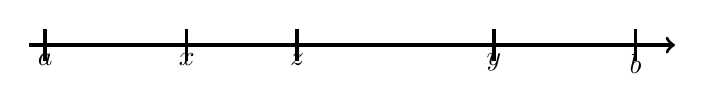
\begin{tikzpicture}[mydrawstyle/.style={draw=black, very thick}, x=1mm, y=1mm, z=1mm]
        \draw[mydrawstyle, ->](-2,30)--(80,30);
        \draw[mydrawstyle](0,28)--(0,32) node[below=5]{$a$};
        \draw[mydrawstyle](18,28)--(18,32) node[below=5]{$x$};
        \draw[mydrawstyle](32,28)--(32,32) node[below=5]{$z$};
        \draw[mydrawstyle](57,28)--(57,32) node[below=5]{$y$};
        \draw[mydrawstyle](75,28)--(75,32) node[below=5]{$b$};
    \end{tikzpicture} \\
    $z:= \lambda x + (1-\lambda)y$

    Так как $x = \lambda x + (1-\lambda)x < \lambda x 
    + (1-\lambda)y < \lambda y + (1-\lambda)y = y$, мы можем точно сказать, что $z$ находится
    между $x$ и $y$.

    $\lambda x + (1-\lambda)y$ - произвольная точка из отрезка $(x, y)$. Если мы позволим $\lambda$
    принимать значения 0 и 1, то формула будет в точности давать отрезок $(x, y)$

    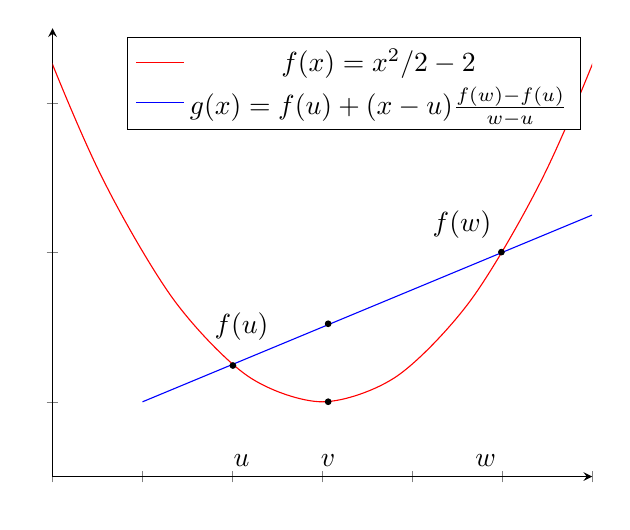
\begin{tikzpicture}
        \draw (2.4cm,1.9cm) node(h) {$f(u)$}
                (2.4cm,0.2cm) node(t) {$u$}
                (5.5cm,0.2cm) node(y) {$w$}
                (5.2cm,3.2cm) node(r) {$f(w)$}
                (3.5cm,0.2cm) node(y) {$v$};
        \begin{axis}[
            xmin=-3,   xmax=3,
            ymin=-3,   ymax=3,
            axis lines = left,
            %xlabel = $x$,
            %ylabel = {$f(x)$},
            yticklabels={,,},
            xticklabels={,,}
        ]
        %Below the red parabola is defined
        \addplot [
            domain=-10:10,
            smooth,
            color=red,
        ]
        {x^2/2 - 2};
        \addlegendentry{$f(x) = x^2/2 - 2$}
        %Here the blue parabloa is defined
        \addplot [
            smooth,
            domain=-2:3,
            color=blue,
        ]
        {x / 2 - 1};
        \addlegendentry{$g(x) = f(u) + (x - u)\frac{f(w) - f(u)}{w - u}$}
        \end{axis}
        \filldraw[black] (2.29cm,1.41cm) circle(1.0pt)
                (5.7cm,2.85cm) circle(1.0pt)
                (3.5cm,0.95cm) circle(1.0pt)
                (3.5cm,1.94cm) circle(1.0pt);
    \end{tikzpicture}

    $v = \lambda u + (1 - \lambda)w$

    Точки $(u, f(u))$ и $(w, f(w))$ - точки пересечения графиков. Формулой для $v$ описывается любая точка 
    из отрезка $(u, w)$. Формула $g(x) = f(u) + (x - u)\frac{f(w) - f(u)}{w - u}$ описывает прямую, соединяющую 
    точки пересечения графиков функций. 
    
    Найдем $g(v)$:
    \begin{equation*}
        \begin{split}
            g(v) &= f(u) + (v - u)\frac{f(w) - f(u)}{w - u} \\
            &= f(u) + \frac{v - u}{w - u}(f(w) - f(u)) \\
            &= f(u) - \frac{v - u}{w - u}f(u) + \frac{v - u}{w - u}f(w) \\
            &= \frac{w - v}{w - u}f(u) + \frac{v - u}{w - u}f(w) 
        \end{split} 
    \end{equation*}
    \[ \lambda = \frac{w - v}{w - u} \Rightarrow 1 - \lambda = \frac{v - u}{w - u} \Rightarrow g(v) = \lambda f(u) + (1 - \lambda)f(w) \]


    Таким образом наше определение выпуклости 
    говорит о том, что точка $(v, f(v))$ на графике функции лежит ниже, чем хорда, соединяющая 
    точки $(u, f(u))$ и $(w, f(w))$.
\end{conj}

\textbf{Пример.} $f(x) = x^2$  строго выпуклая 

$(\lambda x + (1 - \lambda)y)^2 < \lambda x^2 + (1 - \lambda)y^2$

$2 \lambda (1 - \lambda)xy < (\lambda - {\lambda}^2)x^2 + ((1 - \lambda) -
(1 - \lambda)^2)y^2$

$2xy < x^2 + y^2$

\begin{conj}
    $f: \langle a, b \rangle \longrightarrow \R \quad$ вогнутая, если  
    $\forall x, y \in \langle a, b \rangle \quad \forall \lambda \in (0, 1)$

    $f(\lambda x + (1-\lambda)y) \geqslant \lambda f(x) + (1 - \lambda) f(y) \qquad$ \textit{\textbf{выпуклая вверх}}
\end{conj}

\notice $f$ - выпуклая $\Longleftrightarrow (-f)$ - вогнутая

\subsection*{Переформулировка условия выпуклости $\forall u < v < w$ из $\langle a, b \rangle$}

$f(v) \leqslant \frac{w - v}{w - u}f(u) + \frac{v - u}{w - u}f(w)$ \qquad 
$(w - u)f(v) \leqslant (w - v)f(u) + (v - u)f(w)$

\textbf{Свойства: }
\begin{enumerate}
    \item $f, g$ выпуклые на $\langle a, b \rangle \Longrightarrow f + g$ выпуклая на $\langle a, b \rangle$
    \item Если $f$ выпуклая на $\langle a, b \rangle, \alpha > 0 \Longrightarrow \alpha f$ выпуклая на $\langle a, b \rangle$
\end{enumerate}

